\lesson{Structures and Properties of Matter}
We can classify solids with the table below
\begin{tabular-custom}{|c|c|c|}{Classifying Solids}
    Clas of substance & Elements combined & Examples \\ \hline
    ionic & metal + nonmetal & $\ch{NaCl_{(s)}}$, $\ch{CaCO3_{(s)}}$ \\ \hline
    metallic & metal(s) & $\ch{Cu_{(s)}}$, $\ch{CuZn3_{(s)}}$ \\ \hline
    molecular  & nommetal(s) & $\ch{I2_{(s)}}$, $\ch{H2O_{(s)}}$, $\ch{CO2_{(s)}}$ \\ \hline
    covalent network & metalloids/carbon & $\ch{C_{(s)}}$, $\ch{SiC_{(s)}}$, $\ch{SiO2_{(s)}}$ \\ \hline
\end{tabular-custom}

\subsection{Ionic Crystals}
The arrangement of ions within form a \textbf{crystal lattice structure}, see Figure \ref{fig:crystal-lattice}
\begin{bulleted-list}
    \item Relatively hard but brittle
    \item Conducts electricity in liquid state
    \item Forms solutions in water because of dissociation
    \item High melting points
\end{bulleted-list}
\textbf{Ionic bonding} is defined theoretically as the simultaneous attraction of an ion by
surrounding ions of opposite charge.

\begin{figure}[ht!]
    \centering
    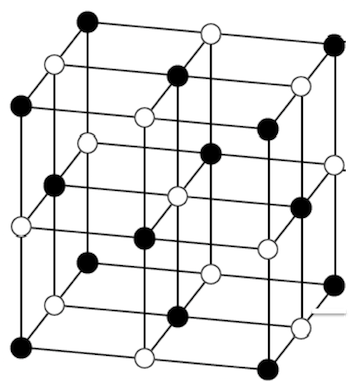
\includegraphics[width=0.4 \textwidth]{../figures/crystal-lattice.png}
    \caption{Crystal lattice structure}
    \label{fig:crystal-lattice}
\end{figure}

\subsection{Metallic Crystals}
All metals have a continuous and very compact crystalline structure. The properties of metals are
the result of the bonding between fixed, positive nuclei and loosely held, mobile valence electrons.
This attraction is not localized or directed between specific atoms, as occurs with ionic crystals.
Instead, the electrons act like a negative ``glue'' around the positive nuclei. 

\begin{bulleted-list}
    \item Low ionization energy of metal atoms to explain loosely held electrons
    \item Empty valence orbitals to explain electron mobility
    \item Electrostatic attraction of positive centers and the negatively charged electron ``sea''
        to explain the strong, nondirectional bonding
\end{bulleted-list}

\begin{important}
    Metals are malleable, ductile, and flexible because the bonding between atoms in metals is
    nondirectional, since the bonding is due to the ``electron sea''.
\end{important}

\begin{figure}[ht!]
    \centering
    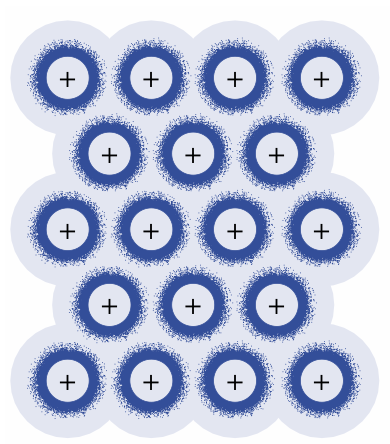
\includegraphics[width=0.4 \textwidth]{../figures/metallic-bonding.png}
    \caption{Each positive charge represents the nucleus and inner electrons of a metal atom,
    surrounded by a mobile ``sea'' of valence electrons.}
    \label{fig:metallic-bonding}
\end{figure}

\subsection{Molecular Crystals}
The intermolecular forces that keep molecular crystals together are the same: LDP, dipole-dipole,
and hydrogen bonding.
\begin{bulleted-list}
    \item These forces are relatively weak compared to ionic and covalent bonds
    \item \textbf{Relatively low-degree hardness of the solids}
    \item \textbf{Low melting points} (compared to ionic compounds)
\end{bulleted-list}

\subsection{Covalent Network Solids}
In most covalent solids, intermolecular forces are quite weak. This is why covalent substances of
low molecular masses are generally gaseous at room temperature.\\

In a few substances, known as \textbf{covalent network solids}, covalent bonds are extended
throughout the crystalline solid. In these cases, the \textbf{entire crystal is held together
by covalent bonds}--the intermolecular and the intramolecular forces are the same. Common examples
are \textbf{diamond} and \textbf{graphite}.
\begin{bulleted-list}
    \item Much \textbf{harder} and \textbf{higher melting/boiling point} that ionic and molecular
        crystals
\end{bulleted-list}

\subsection{Diamond}
A pure carbon compound that has a bonding scheme in which each carbon atom is bonded to 4 other
carbon atoms. This bonding results from $sp^3$ hybridization and gives a \textbf{tetrahedral shape}.
\begin{bulleted-list}
    \item Diamond is \textbf{very hard}
    \item Diamond is a \textbf{non-conductor of electricity}
    \item Diamond melts at $3500^{\circ}\text{C}$
\end{bulleted-list}
In this case, there are no other intermolecular forces, but instead the entire molecule is held
together by covalent bonds--carbon only has a covalent bond to carbon. See Figure \ref{fig:diamond-structure}

\begin{figure}[ht!]
    \centering
    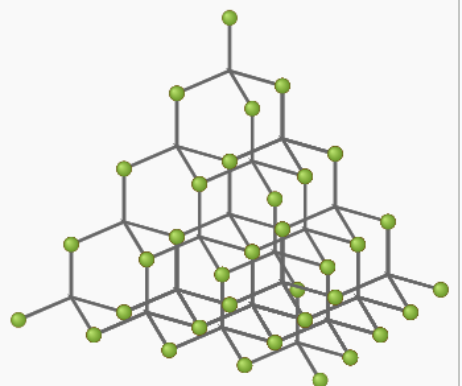
\includegraphics[width=0.3 \textwidth]{../figures/diamond-structure.png}
    \caption{The structure of diamond}
    \label{fig:diamond-structure}
\end{figure}

\subsection{Graphite}
A pure carbon compound that contains carbon atoms that are bonded together in a very different 
way compared to diamonds (see Figure \ref{fig:graphite-structure}. The type of bonding involves the
orbital set $sp^2+p$. Recall that the three $sp^2$ orbitals are directed in a plane at $120^{\circ}$
angles. The p orbital is perpendicular to the plane, directed above and below.\\

Each carbon atom forms strong covalent bonds with three other carbon atoms in a hexagonal arrangement.
The electrons in the $p$ orbitals of the carbon atoms are \textbf{delocalized}
\footnote{
    \textbf{Delocalized:} electrons in a molecule, ion, or solid metal that are not associated
    with a single atom or a covalent bond; electrons that can move throughout atoms in a molecule.
}.
In graphite, the $p$ orbitals in each carbon are equally as close to each other. Therefore,
the delocalized electrons are free to move around.

\begin{bulleted-list}
    \item Graphite \textbf{conducts electricity} because the electrons are moving between the plane
        perpendicular to the traditional $p$ orbital bonding plane (see Figure \ref{fig:graphite-structure})
    \item The bonding \textbf{within layers is very strong} (because they are a covalent network)
        but the bonding \textbf{between layers is very weak} (because they are held with delocalized electrons)
    \item The delocalized electrons moving between covalent planes is not considered to be 
        intermolecular forces
    \item Acts as a lubricant because the covalent network planes slide over one another while
        maintaining the weak intermolecular attractions
\end{bulleted-list}

\begin{figure}[ht!]
    \centering
    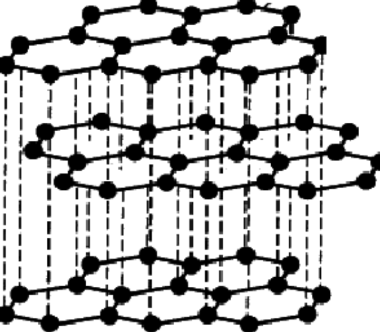
\includegraphics[width=0.3 \textwidth]{../figures/graphite-struct.png}
    \caption{The structure of graphite}
    \label{fig:graphite-structure}
\end{figure}
